%%%% ijcai17.tex

\typeout{IJCAI-17 Instructions for Authors}

% These are the instructions for authors for IJCAI-17.
% They are the same as the ones for IJCAI-11 with superficical wording
%   changes only.{\tiny {\tiny {\tiny {\tiny }}}}

\documentclass{article}
% The file ijcai17.sty is the style file for IJCAI-17 (same as ijcai07.sty).
\usepackage{ijcai17}
 \usepackage{amsmath}
 \usepackage{graphicx}
 \usepackage{makecell}
 \usepackage{listings}
 \usepackage{xcolor} 
% Use the postscript times font!
\usepackage{times}

% the following package is optional:
%\usepackage{latexsym} 

% Following comment is from ijcai97-submit.tex:
% The preparation of these files was supported by Schlumberger Palo Alto
% Research, AT\&T Bell Laboratories, and Morgan Kaufmann Publishers.
% Shirley Jowell, of Morgan Kaufmann Publishers, and Peter F.
% Patel-Schneider, of AT\&T Bell Laboratories collaborated on their
% preparation.

% These instructions can be modified and used in other conferences as long
% as credit to the authors and supporting agencies is retained, this notice
% is not changed, and further modification or reuse is not restricted.
% Neither Shirley Jowell nor Peter F. Patel-Schneider can be listed as
% contacts for providing assistance without their prior permission.

% To use for other conferences, change references to files and the
% conference appropriate and use other authors, contacts, publishers, and
% organizations.
% Also change the deadline and address for returning papers and the length and
% page charge instructions.
% Put where the files are available in the appropriate places.

\title{Project 2: Image Recovery}
\author{Yufeng Yuan\\ 
yy208@duke.edu}

\begin{document}

\maketitle

\begin{abstract}
  In this project, for a given image, we need to sample some pixel points in the image to recover the original image. The sample points should be segmented into training set and test set randomly and only the training set would be used before finishing cross validation. With Discrete Cosine Transformation and the sample points, an under-determined linear system could be formed which could be solved by Orthogonal Match Pursuit. Then cross validation could be applied to find the best hyper-parameter. With the optimal hyper-parameter, the sparse solution could be obtained by Orthogonal Match Pursuit algorithms. Inverse Discrete Cosine Transform could be applied next to recover the original image. The recovery quality is measured by the mean square error.

\end{abstract}

\section{Overview}

First, I implemented a function for random sampling with a Matlab built-in function randomperm which generates random integer sequence, this approach ensures that there's no repeated points in the samples. For OMP Solver function, first half of it is to generate the under-determined linear system of Discrete Cosine Transform and the second half is to solve the linear system with a given lambda by OMP algorithms. Also, this function is implemented with some matrix operation techniques to improve the running efficiency. For the implementation of cross validation, all the sample points will first be segmented into training set and test set randomly. Then, the OMP solver and inverse DCT will be applied based on the training set to recover the image. By comparing the recovery quality, the optimal hyper-parameter could be found by doing cross validation for 20 times. The last function is Inverse Discrete Cosine Transform, with the optimal hyper-parameter, the image could eventually be recovered by IDCT. Note: The whole project was done in Octave environment, there might be some capability issues when running in Matlab.

\section{Mathematical Formulation}
This section consists of two subsections, the first is how the linear system is obtained and the second is how the  Orthogonal Match Pursuit algorithms is implemented.
\subsection{Linear System}
A 2-D image can be mapped to frequency domain by Discrete Cosine Transform (DCT)
$$
G(u,v)=
\sum^P_{x=1}\sum^Q_{y=1}a_u \cdot b_v \cdot g(x,y) \cdot cos \frac{\pi(2x \!-\! 1)(u\!-\!1)}{2 \cdot P}
$$
$$
\cdot cos \frac{\pi (2y \!-\! 1)(v\!-\!1)}{2 \cdot Q}
$$

$$
x,u \in \{1,2,...P\}\quad
y,v \in \{1,2,...Q\}\\
$$

$$
a_u=\left\{
\begin{aligned}
\sqrt \frac{1}{P} &\ (u=1)\\
\sqrt \frac{2}{P} &\ (2 \leq u \leq P)\\
\end{aligned}
\right.
$$
$$
b_v=\left\{
\begin{aligned}
\sqrt \frac{1}{Q} &\ (v=1)\\
\sqrt \frac{2}{Q} &\ (2 \leq v \leq Q)\\
\end{aligned}
\right.
$$
Reversely, a 2-D image can also be uniquely determined by Inverse Discrete Cosine Transform (IDCT), if all DCT coefficients are known.
$$
g(x,y)=
\sum^P_{u=1}\sum^Q_{v=1}a_u \cdot b_v \cdot G(u,v) \cdot cos \frac{\pi(2x\!-\!1)(u\!-\!1)}{2 \cdot P}\\
$$
$$
\cdot cos \frac{\pi (2y\!-\!1)(v\!-\!1)}{2 \cdot Q}
$$
We can find the approximate solution of DCT coefficients by sampling a 2-D image at M spatial locations and form a set of M linear equations.

$$
g(x_1, y_1) = \sum^P_{u=1}\sum^Q_{v=1}a_u \cdot b_v \cdot G(u,v) \cdot cos \frac{\pi(2x_1-1)(u-1)}{2 \cdot P}
$$
$$
\cdot cos \frac{\pi (2y_1-1)(v-1)}{2 \cdot Q}\\
$$
$$
g(x_2, y_2) = \sum^P_{u=1}\sum^Q_{v=1}a_u \cdot b_v \cdot G(u,v) \cdot cos \frac{\pi(2x_2-1)(u-1)}{2 \cdot P}
$$
$$
\cdot cos \frac{\pi (2y_2-1)(v-1)}{2 \cdot Q}
$$
$$
\cdot \cdot \cdot \cdot\\
$$
$$
g(x_M, y_M) = \sum^P_{u=1}\sum^Q_{v=1}a_u \cdot b_v \cdot G(u,v) \cdot cos \frac{\pi(2x_M-1)(u-1)}{2 \cdot P}
$$
$$
\cdot cos \frac{\pi (2y_M-1)(v-1)}{2 \cdot Q}
$$
Rewrite the linear equations in matrix form, which is an under-determined linear system. For simplicity, we use 
$ C_{m,u,v}$ to denote $ a_u \cdot b_v \cdot cos \frac{\pi(2x_m-1)(u-1)}{2 \cdot P} \cdot cos \frac{\pi (2y_m-1)(v-1)}{2 \cdot Q}$
$$
\begin{bmatrix}
g(x_1,y_1)\\
g(x_2,y_2)\\
\vdots\\
g(x_M,y_M)\\
\end{bmatrix}=
$$

$$
\begin{bmatrix}
C_{1,1,1} & C{1,1,2} & \cdots & C_{1,P,Q-1} & C_{1,P,Q}\\
C_{2,1,1} & C{2,1,2} & \cdots & C_{2,P,Q-1} & C_{2,P,Q}\\
&&\vdots\\
C_{M,1,1} & C{M,1,2} & \cdots & C_{M,P,Q-1} & C_{M,P,Q}\\
\end{bmatrix}
\cdot
\begin{bmatrix}
G(1,1)\\
G(1,2)\\
\vdots\\
G(P,Q)
\end{bmatrix}
$$
This is an under-determined linear system, and  Orthogonal Match Pursuit (DCT) algorithms described below is one of the ways to solve it.
\subsection{The Implementation of OMP Algorithms}
These are the goal function and constraint for this problem
$$
\min_\alpha \Vert A \alpha - B\Vert^2_2
$$
$$
S.T. \Vert \alpha \Vert_0 \leq \lambda
$$
Step 1: Set F = B, $ \Omega = \{\} $ and p = 1
$$
$$
Step 2: Calculate the inner product values $ \theta_i = <A_i, F> $
$$
$$
Step 3: Identify the index s for which $ \vert \theta_s\vert $ takes the largest number
$$
$$
Step 4: Update $\Omega $ by $\Omega = \Omega \cup \{s\}$
$$
$$
Step5: Approximate F by the linear combination of $ \{ A_i, i \in \Omega \} $
$$
$$
$$\min_{a_i,j \in \Omega} \Vert \sum_{i\in\Omega }\alpha_i \cdot A - B \Vert_2^2$$
$$
$$
Step 6: Update F
$$
$$
$$F = B - \sum_{i \in \Omega}\alpha_i \cdot A$$
$$
$$
Step 7: if p $\le \lambda$, p = p + 1 and go to Step 2. Otherwise, stop.
$$
$$
$\alpha_i = 0 (i \notin \Omega)$
$$
$$
\section{Experimental Results}

\subsection{Small Test Image}

The block size of this image is 8 by 8, the error shown is after median filtering.


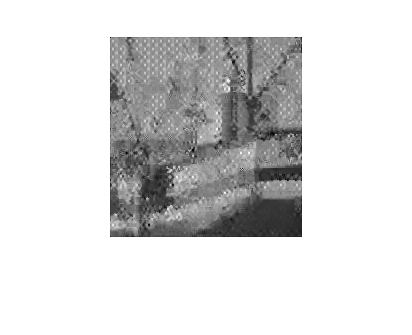
\includegraphics[width=2in,height=2in]{1-10.png}
\vspace{-0.5in}

Sample Size = 10, Mean Square Error = 1563.0

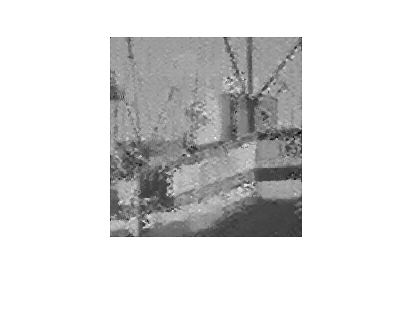
\includegraphics[width=2in,height=2in]{1-20.png}
\vspace{-0.5in}

Sample Size = 20, Mean Square Error = 1374.4

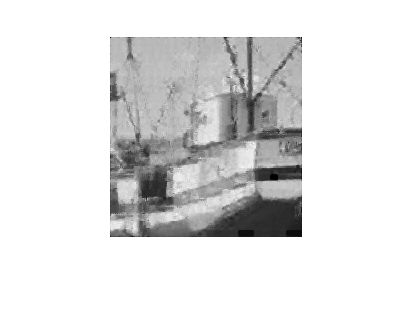
\includegraphics[width=2in,height=2in]{1-30.png}
\vspace{-0.5in}

Sample Size = 30, Mean Square Error = 1340.2

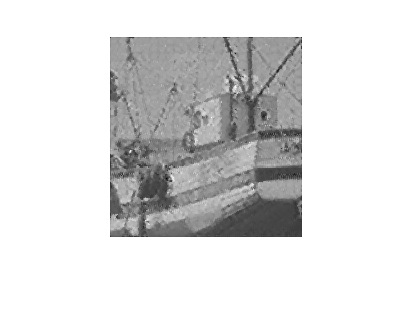
\includegraphics[width=2in,height=2in]{1-40.png}
\vspace{-0.5in}

Sample Size = 40, Mean Square Error = 1157.7

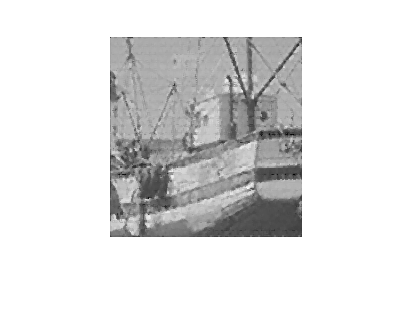
\includegraphics[width=2in,height=2in]{1-50.png}
\vspace{-0.5in}

Sample Size = 50, Mean Square Error = 1090.7

\subsection{Large Test Image}
The block size of this image is 16 by 16, the error shown here is after median filtering.

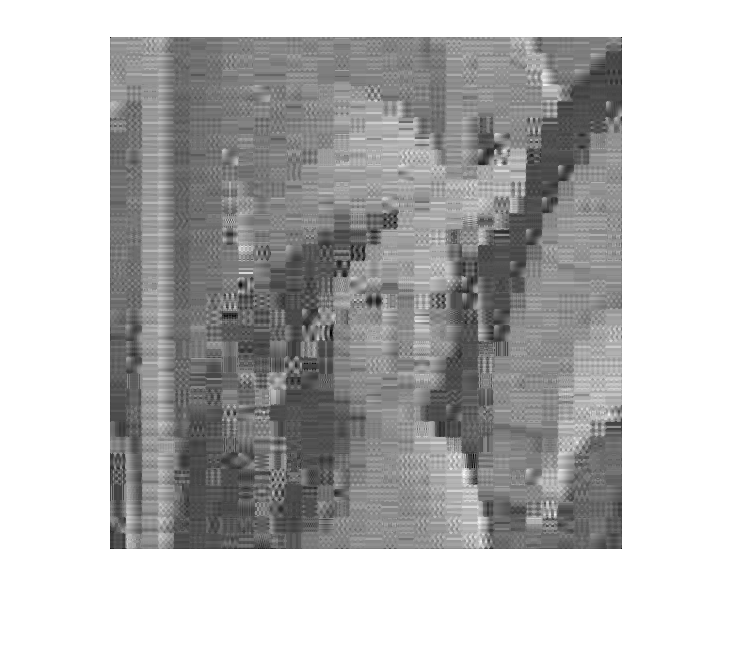
\includegraphics[width=2in,height=2in]{2-10.png}
\vspace{-0.1in}

Sample Size = 10, Mean Square Error = 742.9

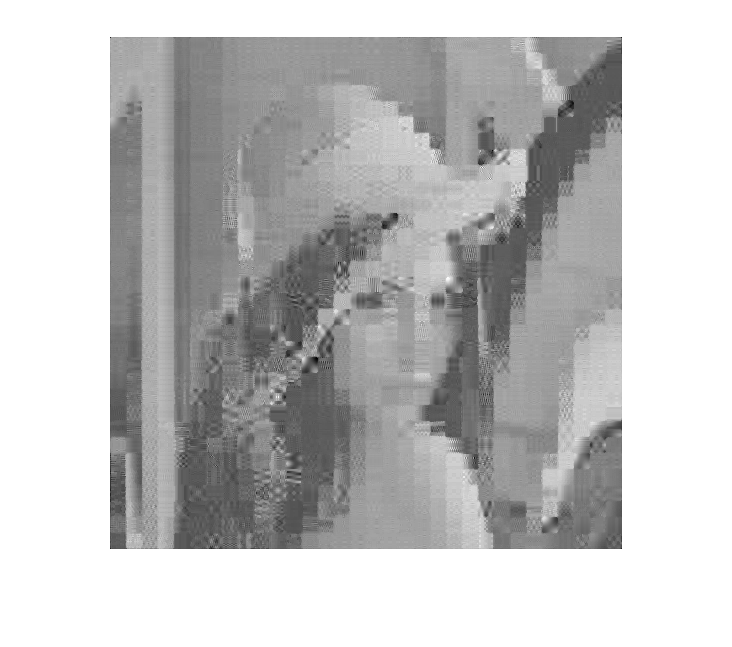
\includegraphics[width=2in,height=2in]{2-30.png}
\vspace{-0.1in}

Sample Size = 30, Mean Square Error = 638.9
 
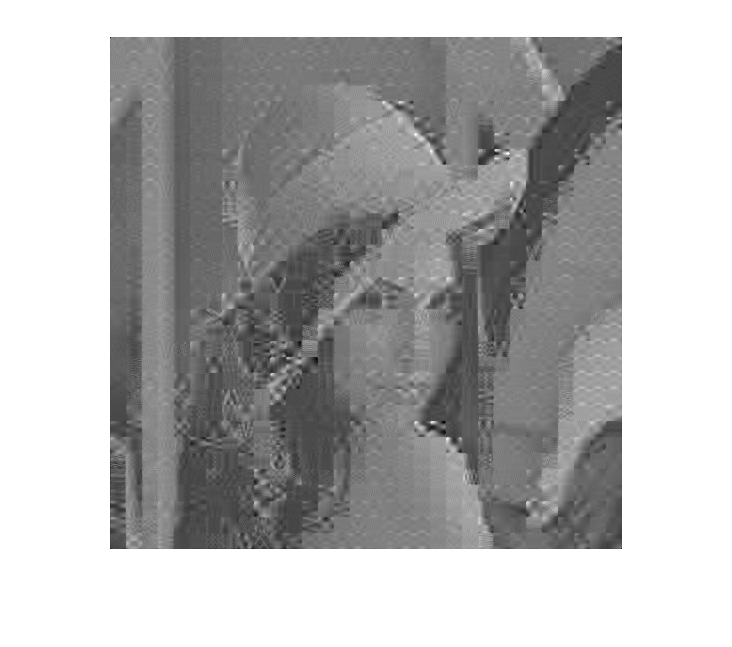
\includegraphics[width=2in,height=2in]{2-50.png}
\vspace{-0.1in}

Sample Size = 50, Mean Square Error = 598.9

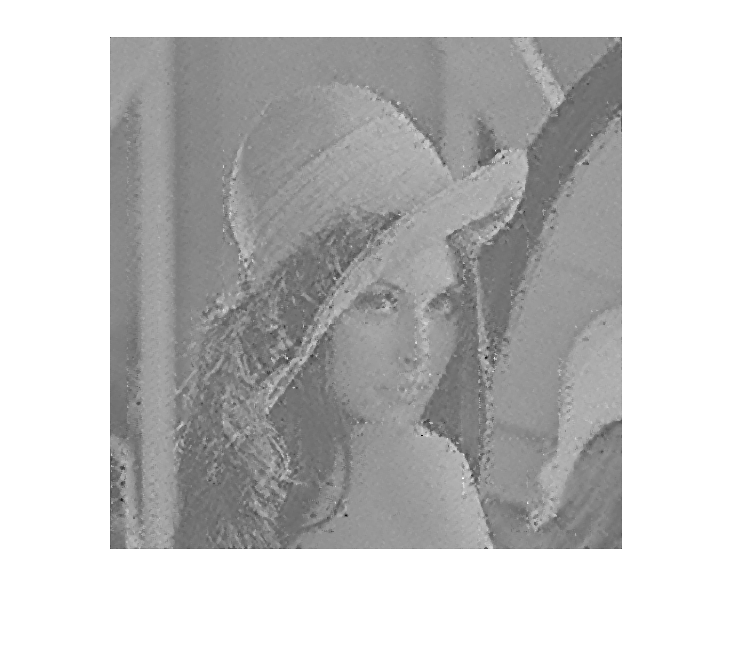
\includegraphics[width=2in,height=2in]{2-100.png}
\vspace{-0.1in}

Sample Size = 100, Mean Square Error = 540.1

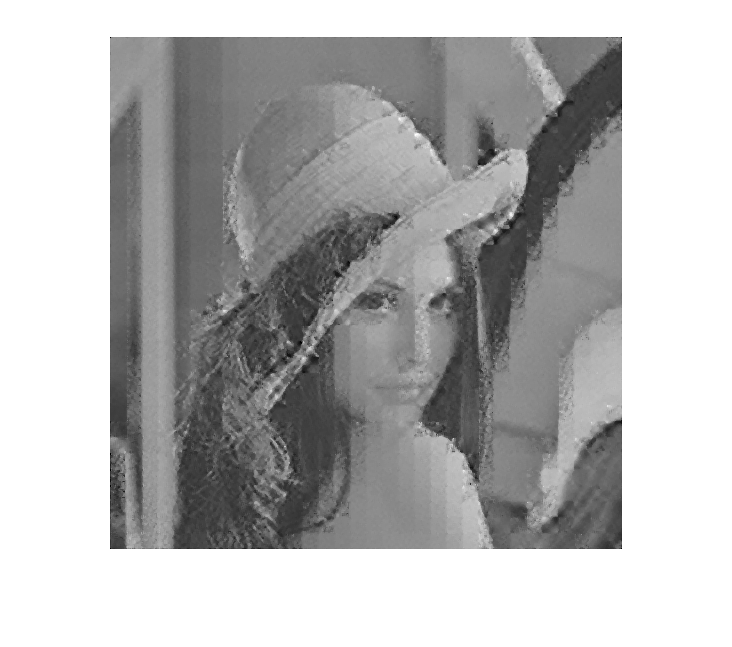
\includegraphics[width=2in,height=2in]{2-150.png}
\vspace{-0.1in}

Sample Size = 150, Mean Square Error = 544.4

\subsection{Cross Validation}

In cross validation, we need to find the optimal lambda which is a hyper-parameter for OMP algorithms. We use lambda ranging from 5 to 50. More specifically, lambda = [5, 10, 15, 20, 30, 50]. For better comparison, we use the same lambda setting for both images.
The following diagrams are the optimal lambda found by cross validation, the first figure is the small one and the second figure is the large one. In general, the optimal lambda increases with the sample number.

\vspace{1.5em}

\begin{tabular}{|r|r|}
	\hline
	\makecell{Samples} & \makecell{Lambda}  \\ \hline
	
	10 & 5 \\
	20 & 20 \\ 
	30 & 10 \\ 
	40 & 30 \\ 
	50 & 50 \\  
	\hline
	
\end{tabular}

\vspace{1.5em}

\begin{tabular}{|r|r|}
	\hline
	\makecell{Samples} & \makecell{Lambda}  \\ \hline
	
	10 & 5 \\
	30 & 5 \\ 
	50 & 10 \\ 
	100 & 50 \\ 
	150 & 50 \\  
	\hline
	
\end{tabular}
\vspace{5em}
\subsection{Recovery Error}
The first diagram is for the small test image whose sample numbers are 10, 20, 30, 40 and 50. The second diagram is for the large test image whose sample numbers are 10, 30, 50, 100 and 150. Error 1 is the mean square error after median filtering, while error 2 is the mean square error before median filtering.

\vspace{1.5em}

\begin{tabular}{|r|r|r|}
	\hline
	\makecell{Samples} & \makecell{Error 1} & \makecell{Error 2} \\ \hline
	
	10 & 1563.0 & 2320.8\\
	20 & 1374.4 & 2168.2\\ 
	30 & 1340.2 & 1520.8\\ 
	40 & 1157.7 & 3007.0\\ 
	50 & 1090.7 & 3374.9\\  
	\hline
	
\end{tabular}

\vspace{1.5em}

\begin{tabular}{|r|r|r|}
	\hline
	\makecell{Samples} & \makecell{Error 1} & \makecell{Error 2} \\ \hline
	
	10 & 742.9 & 1049.8\\
	30 & 638.9 & 790.1\\ 
	50 & 598.9 & 652.8\\ 
	100 & 540.1 & 984.0\\ 
	150 & 544.4 & 666.9\\  
	\hline
	
\end{tabular}
\vspace{1.5em}
\section{Discussion}
\subsection{Factors that Impact the Recovery Quality}
\subsubsection{Sample Number}
With the increase of sample number, the improvement of the recovery quality could be observed here. In our settings, the quality improvement is more obvious at first several times of increasing sample points, after that, the improvement becomes less obvious. However, the cost of more sample points is longer sampling process and computation. It hard to find the optimal sample number to balance the computation time and recovery quality because it's very problem-dependent.
\subsubsection{Lambda for OMP Algorithms}
According to the figure above, lambda chosen by cross validation is different with different sample numbers. For different sample numbers, there are different lambdas that fit the problem optimally. However, the cross validation process is very computational-expensive and the how to choose the range of lambdas is also experience-dependent. 
\subsubsection{Block Size}
Though the block size is given in this project, an appropriate block size is crucial to image recovery which is why we have two different settings for two test images. For each block, we need to find the sparse solution by OMP algorithms. If the block size is too large, the solution may not be sparse. If the block size is too small, the recovery quality may not be that good.
I've tried several different block sizes, and they did perform worse than the original setting. The errors shown below are the large test image with sample number 50 and median filtering under different block size settings. It seems that smaller block size may perform better, but the cost is long computation time.

\begin{tabular}{|r|r|}
	\hline
	\makecell{Block Size} & \makecell{Error}  \\ \hline
	
	8 & 494.2 \\
	16 & 598.9 \\ 
	32 & 781.7 \\ 
	64 &  1571.3\\ 
	\hline
	
\end{tabular}
\subsection{Limits of This approach}
\subsubsection{Computational Complexity}
This algorithms consists of many loops inside, the whole algorithms has high computational complexity though some of the computation could be accelerated by matrix operation. The time required for computation increases rapidly with the increase of problem size, which makes this approach unable to handle high-resolution images.
\subsubsection{Hyper-Parameters}
This approach also consists of a lot of hyper-parameters like block size, and lambda for OMP algorithms. Those parameters should be carefully tuned because these parameters are critical to the recovery quality. However, this is very time-consuming and experience-dependent . 

\subsection{Improvement of Running Efficiency}
The bottleneck of this approach is that there are so many loop in it, and part of the loop could be rewritten as matrix operation form. For example, the generation of DCT coefficients linear system, I implemented it without any loop which greatly accelerated the computation. The code is shown below.
\begin{lstlisting}[language=matlab]
[b,n,m] = size(points);
block = 1:1:blockSize;
x = points(1,:,2)'; y = points(1,:,3)';
matrix1 = cos(pi*(2*x-1)*(block-1)/(2*blockSize));
matrix2 = cos(pi*(2*y-1)*(block-1)/(2*blockSize));
matrix1 = repmat(matrix1, 1, blockSize);
matrix2 = kron(matrix2, ones(1, blockSize));
matrix = matrix1 .* matrix2;
matrix /= blockSize; matrix *= 2;
matrix(1,:) /= sqrt(2);
matrix(:,1) /= sqrt(2);
\end{lstlisting}

\end{document}

